\chapter{Theory}
\label{chap: Theory}

\section{Theory Overview}
首先选择其中两张照片,通过特征点匹配基础矩阵或本征矩阵的求解得到两个拍摄视角的相对位姿,然后使用三角化得到对应特征点的三维点云。对于第三张图,我们可通过相机位姿估算的方式求解其姿态和位置。在这里用的方法是通过第一张图片与第三张图片的特征点与三角化的三维点云的3D-2D匹配关系,利用RANSAC方法实现第三个视角的相机位置姿态估算。

\section{Theory Detail}
\subsection{相机内参标定}
通过MATLAB工具箱进行相机内参标定,需要用同一个相机对某个图案(这里选择黑白棋盘)拍摄多个位姿的图片,按照官方示例进行标定。其中拍摄的20张黑白棋盘的位姿图片如图4所示:

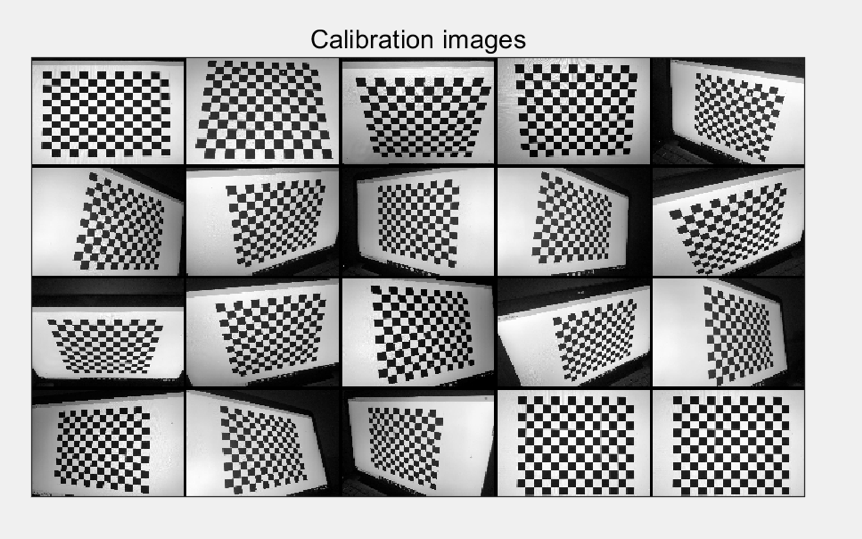
\includegraphics[width=0.7\textwidth]{figures/Picture1.png}
\subsection{去畸变}
对于想要的无畸变的目标图像,从已畸变的图像找出对应的像素,将该像素颜色填入目标图像,以此构建像素映射完成去畸变图像

\subsection{SURF}
SURF(Speeded Up Robust Features, 加速稳健特征) 是一种稳健的图像识别和描述算法。它是SIFT的高效变种,也是提取尺度不变特征,算法步骤与SIFT算法大致相同,但采用的方法不一样,要比SIFT算法更高效(正如其名)。SURF使用海森(Hesseian)矩阵的行列式值作特征点检测并用积分图加速运算;SURF 的描述子基于 2D 离散小波变换响应并且有效地利用了积分图

算法步骤:
\begin{enumerate}
    \item \textbf{特征点检测}:SURF使用Hessian矩阵来检测特征点,该矩阵是x,y方向的二阶导数矩阵,可测量一个函数的局部曲率,其行列式值代表像素点周围的变化量,特征点需取行列式值的极值点。用方型滤波器取代SIFT中的高斯滤波器,利用积分图(计算位于滤波器方型的四个角落值)大幅提高运算速度
    \item \textbf{特征点定位}:与SIFT类似,通过特征点邻近信息插补来定位特征点
    \item \textbf{方向定位}:通过计算特征点周围像素点x,y方向的哈尔小波变换,并将x,y方向的变换值在xy平面某一角度区间内相加组成一个向量,在所有的向量当中最长的(即x、y分量最大的)即为此特征点的方向。
    \item \textbf{特征描述子}:选定了特征点的方向后,其周围相素点需要以此方向为基准来建立描述子。此时以$5\times5$个像素点为一个子区域,取特征点周围$20\times20$个像素点的范围共16个子区域,计算子区域内的$x$、$y$方向(此时以平行特征点方向为x、垂直特征点方向为$y$)的哈尔小波转换总和$\sum dx$、$\sum dy$与其向量长度总和$\sum \vert dx\vert$、$\sum\vert dy\vert$共四个量值,共可产生一个64维的描述子。
\end{enumerate}

\subsection{RANSAC}

在经典的RANSAC流程中,目标函数$C$可以被看作:在第k次迭代过程中,在当前变换参数$\theta_k$作用下,数据集中满足变换参数的点的个数,也就是在当前变换条件下类内点的个数,而RANSAC就是最大化$C$的的过程。而判断当前某个点是否为类内需要一个阈值$t$。

在迭代的过程中,当前变换参数$\theta$的计算需要$U$中的一个子集$ I $来计算,RANSAC是一个随机从$U$中采样一个子集,然后对参数“估计-确认”的循环。每一个子集应是一个大小为$m$ 的最小采样。所谓最小采样,就是$m$ 的大小刚好满足计算$\theta$的个数即可。
在置信度为$\eta_0$的条件下,在循环过程中,至少有一次采样,使得采样出的$m $个点均为类内点,这样才能保证在循环的过程中,至少有一次采样能取得目标函数的最大值。因此,采样次数$k$应该满足以下条件:

$$
    k>\frac{\log(1-\eta_0)}{\log(1-\epsilon^m)}
$$

这里除了置信度$\eta_0$外,$m $为子集大小,$\epsilon$为类内点在$u$中的比例,其中置信度一般设置为[0.95, 0.99]的范围内。然而在一般情况下,$\epsilon$显然是未知的,因此 $\epsilon$可以取最坏条件下类内点的比例,或者在初始状态下设置为最坏条件下的比例,然后随着迭代次数,不断更新为当前最大的类内点比例。

\subsection{三角化进行点云重构原理}
三角化的过程即为在已知两个成像平面中对应的点位置$(x,x^\prime)$的情况下,如果知道两个成像视角的相机矩阵$(y,y^\prime)$,就可以重构出该对应点在三维空间中的位置